\documentclass{article}

\usepackage{graphicx}
\usepackage{amsmath}
\usepackage{amssymb}
\usepackage{hyperref}
\usepackage{biblatex} %Imports biblatex package
\usepackage{amsmath}
\usepackage{algorithm}
\usepackage{algpseudocode}
% \usepackage{float}
\usepackage[margin=1.5in]{geometry}
\addbibresource{sources.bib} %Import the bibliography file

\title{A Blockchain Based Public Health Record System}
\author{
    \begin{tabular}{c}
        Ghanem Ghanem \\
        \small University of Windsor \\
        \small \href{mailto:ghanemg@uwindsor.ca}{ghanemg@uwindsor.ca}
    \end{tabular}
    \and 
    \begin{tabular}{c}
        Kumail Raza \\
        \small University of Windsor \\
        \small \href{mailto:raza11g@uwindsor.ca}{raza11g@uwindsor.ca}
    \end{tabular}
}
\date{\today}

\begin{document}

\maketitle

\begin{abstract}
Blockchain technology has attracted significant attention in various industries for its potential to revolutionize traditional methods of data storage and management. In the healthcare industry, blockchain technology can be applied to public health record (PHR) management to provide patients with greater autonomy over their personal health information. This paper explores the benefits and drawbacks of using blockchain technology for PHR management and presents an implementation of a prototype blockchain-based PHR system. Our prototype includes a decentralized blockchain structure, encryption of sensitive data using RSA, and networking infrastructure. We highlight the limitations and challenges that need to be overcome by our prototype and the industry as a whole for practical use cases.
\end{abstract}
% TODO: add keywords


\section{Introduction}
Managing health records is a critical aspect of the healthcare industry. Traditional methods of health record management are limited by factors such as centralized control, limited patient autonomy, and security risks. The growth of blockchain technology has provided a promising alternative to these challenges by introducing a decentralized, secure, and transparent method of health record management. This work aims to explore the potential of using a blockchain based public health record system (PHR). We present a prototype implementation of a blockchain-based PHR system, and discuss the challenges and limitations of our implementation that need to be addressed for practical use cases. Additionally, we focus on analyzing the benefits and drawbacks of using blockchain technology for PHR implementations, the nature of decentralization in PHRs, the use of encryption standards like RSA to safeguard patient privacy, and networking infrastructure.

\section{Implementation}
Our implementation of a PHR system included the design and production of a prototype with much of the core functionality completed. Our prototype allows for the generation of encryption key pairs (private and public keys), the addition of records encrypted using the previously mentioned keys, and the ability to decrypt and view records. Additionally, it features rudimentary networking capacities in order to showcase how a network could be built after expanding upon it.

\subsection{Blockchain Structure}
We decided to have individual blocks represent a single health record. A single health record is meant to be used to represent a single visit a patient has with a health care provider. 

\subsubsection{Block Class}
Every block on the blockchain is represented as an instance of the "Block" class which is defined with the following fields.
\begin{itemize}
  \item \texttt{doctor} - the name of the patient's doctor provided in the record.
  \item \texttt{diagnosis} - the patient's diagnosis data provided in the record.
  \item \texttt{symptoms} - the patient's symptoms listed in the provided record.
  \item \texttt{treatment} - the prescribed treatment for the patient as listed in the record.
  \item \texttt{prescription} - the drug prescription(s) provided to the patient by the doctor as listed in the record.
  \item \texttt{uuid} - a unique identifier generated before the block is added to the chain, used to identify the block after it has been added.
  \item \texttt{transaction} - a unique identifier for the transaction, created during mining.
  \item \texttt{timestamp} - a timestamp string generated during mining.
  \item \texttt{index} - the index of the block within the chain, it starts at zero and is incremented by one for every additional block.
  \item \texttt{previous\_hash} - SHA-256 hash of the previous block's fields.
\end{itemize}

Aside from the constructor, the "Block" class contains a single additional function. The \texttt{create\_hash()} function returns the SHA\-256 hash of a string generated from the values of all of the fields listed above. Due to the nature of SHA-256, this value is unique for every block. The value returned by this function is used to link adjacent blocks to each other through the \texttt{previous\_hash} field, as described above.

\subsubsection{Blockchain Class}
There exists a \texttt{Blockchain} class which contains reference to a single block. This block is referred to as the \texttt{genesis\_block} and is the first block in the chain. It contains dummy values and can be though of as the head of a linked list, with the linked list being the entirety of the block chain. The first real block is linked with the genesis block, and subsequent blocks are linked to next the block adjacent to them.

Additionally, the blockchain class contains various aspects relating to networking. Further discussion of this can be found in Section \ref{networking}. 

\begin{figure}[h]
\centering
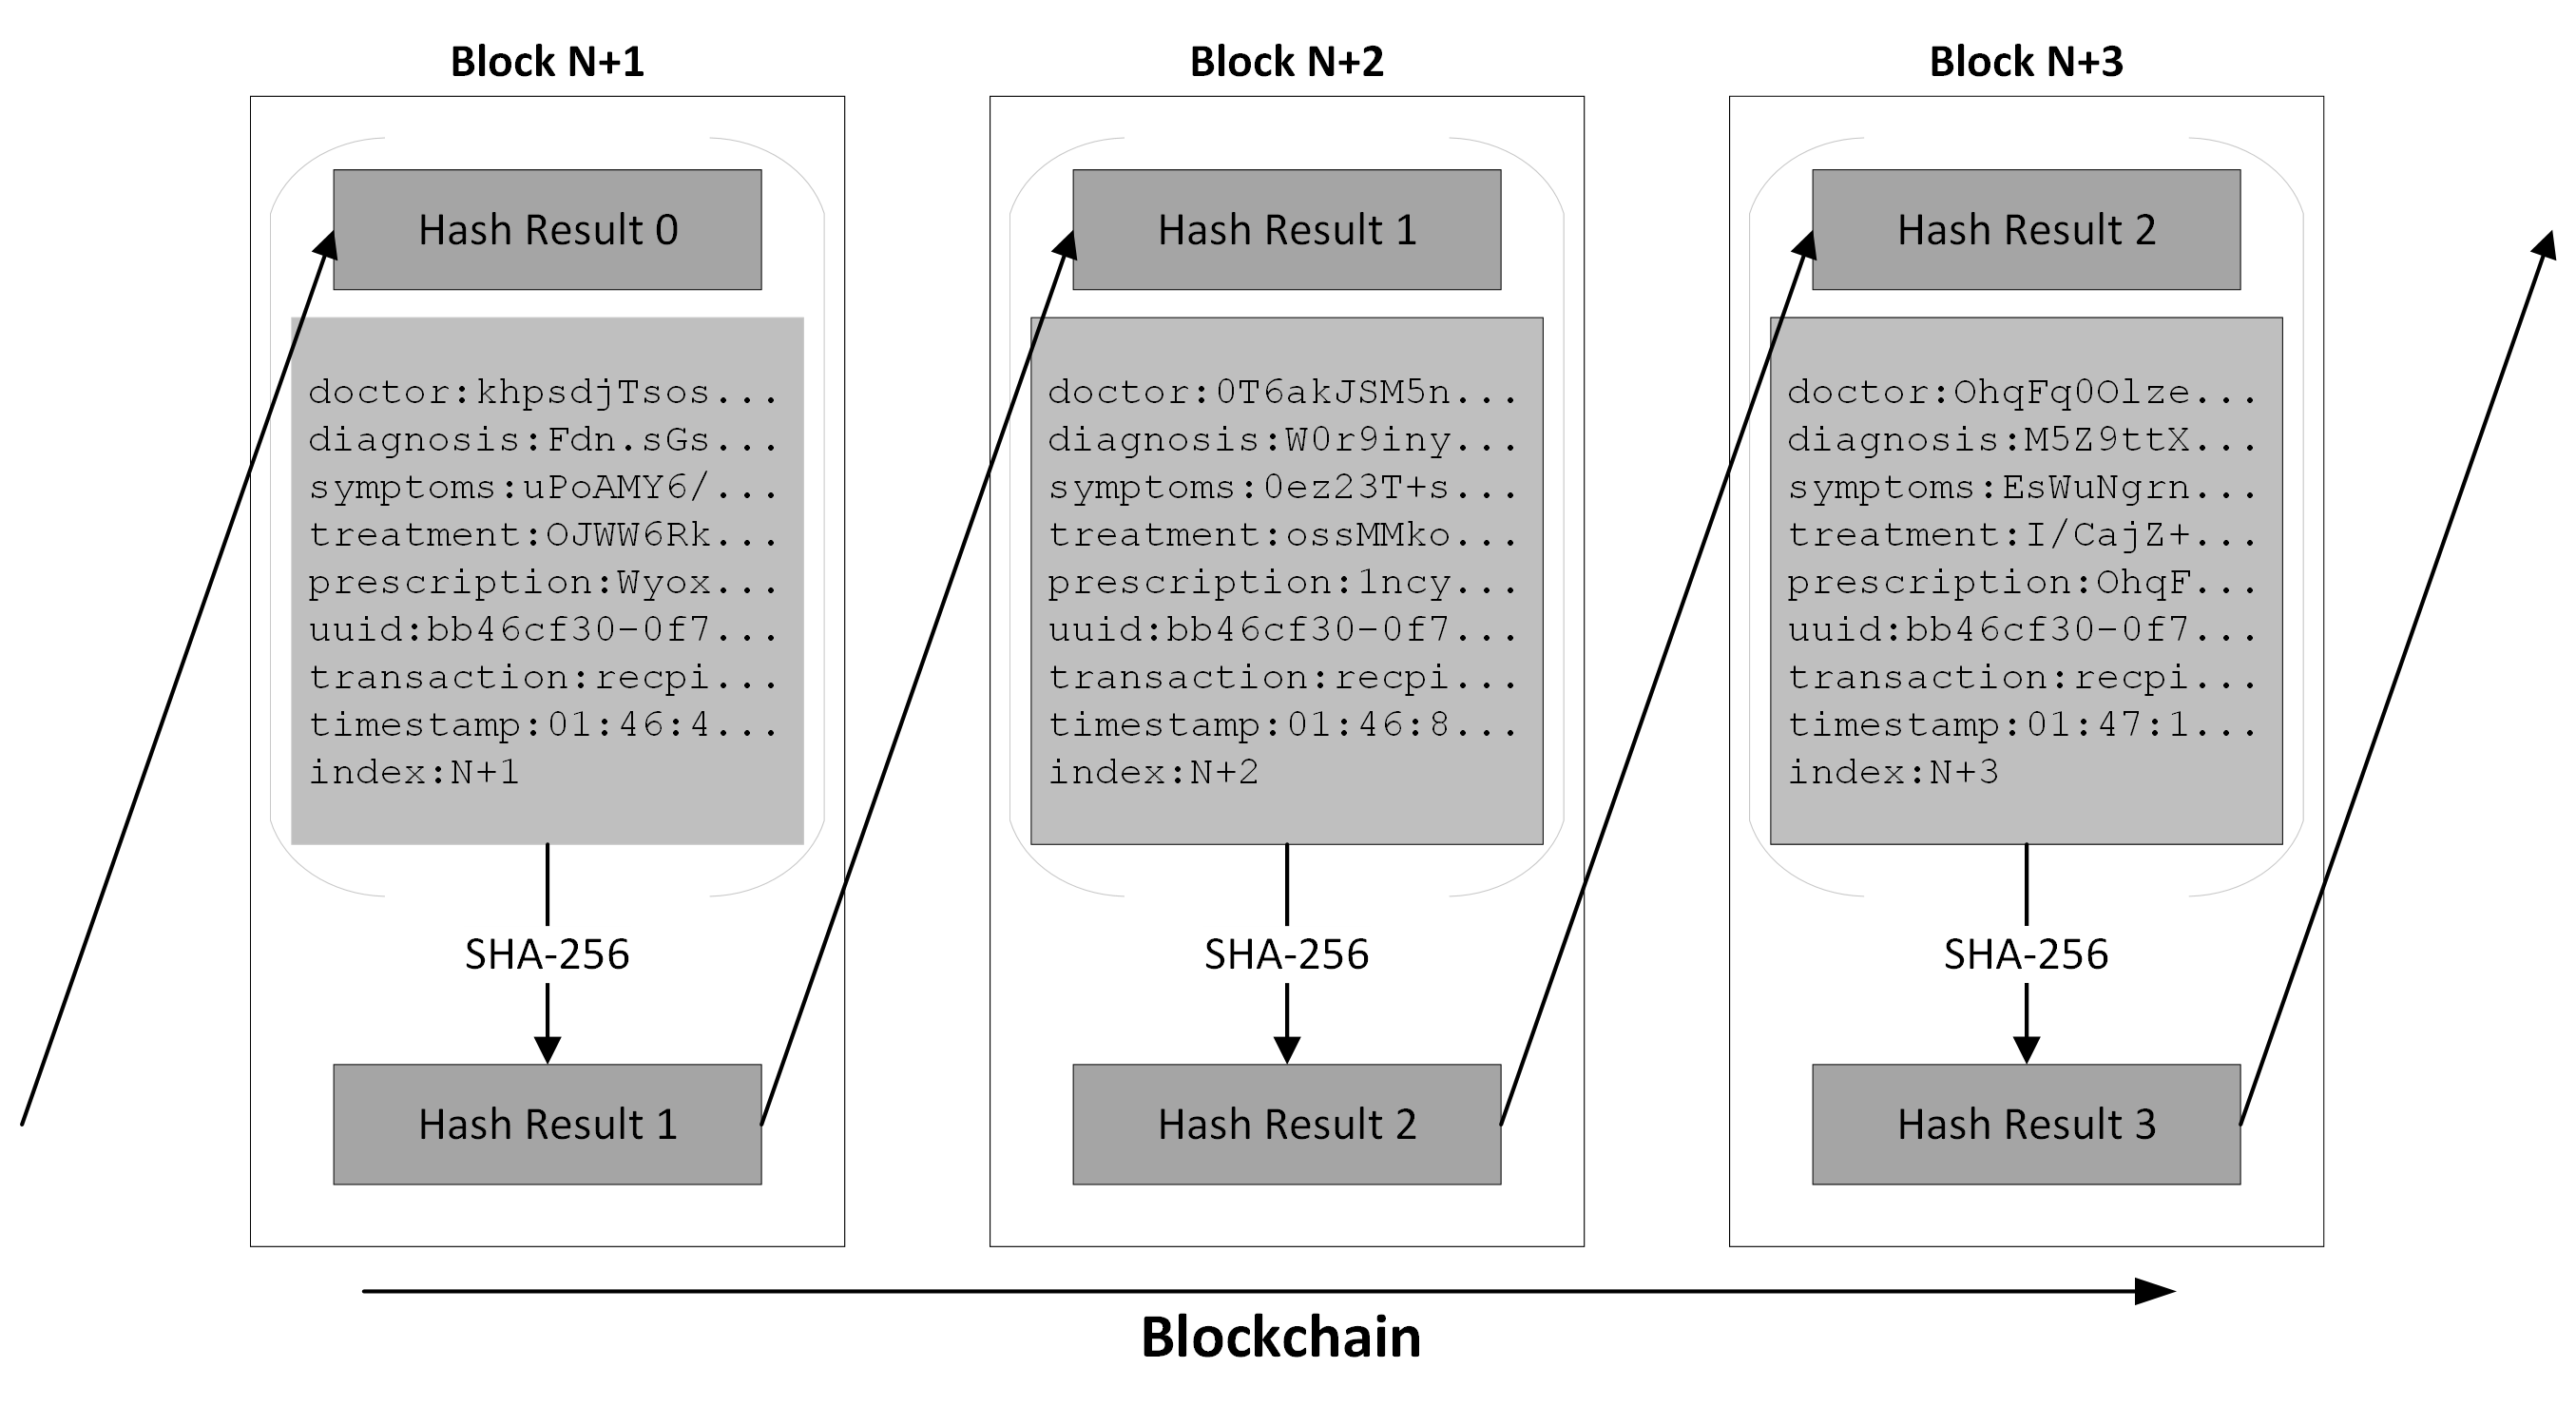
\includegraphics[width=\textwidth]{images/4990_blockchain_structure.png}
\caption{This diagram shows the structure of our public health record blockchain. Each block contains a single record made up of multiple fields, including encrypted strings of information inputted by doctors. These encrypted strings are only readable with the correct public key. The hash of the string data is used as a pointer to the next block.}
\label{fig:encryption_encryption}
\end{figure}

% TODO:
%!!!ADD MORE HERE!!! add other subsections beyond blockchain structure and also add more sub-subsections explaining blockchain structure further.

\subsection{Encryption}
Patient privacy is a critical aspect of a functional PHR implementation. In order to preserve the dignity and privacy of patients, it is vital that their data is never provided to anyone else without explicit consent. This poses a challenge to our decentralized blockchain implementation, where anyone is mean to be able to host a copy of all of the data contained on the blockchain. This also applies to healthcare providers - we decided that patients should be able to control what, if any, providers have access to their data.

The solution that we arrived at for this problem was to use a form of asymmetric encryption to encrypt all sensitive fields before they are added to the blockchain. We decided to use RSA for our prototype due to simplicity \cite{menezes_van_oorschot_vanstone_2001}, however there are potentially more suitable encryption standards that should be used for a production use case as discussed in \ref{limitations:encryption}. % consider changing this citation to fit more naturally in the paragraph. New sentence?

When a patient's record is added to the blockchain, we require the public encryption key associated with the given patient to be provided. The plain-text provided for the record is then encrypted using the provided public key. Unreadable cipher-text is what is then added to the blockchain.

The cipher-text that is then stored in the block can only be decrypted using the private key that is associated with the public key used to initially encrypt it. This makes it so that the data on the blockchain is only available to those with the corresponding private key.

\begin{figure}[h]
\centering
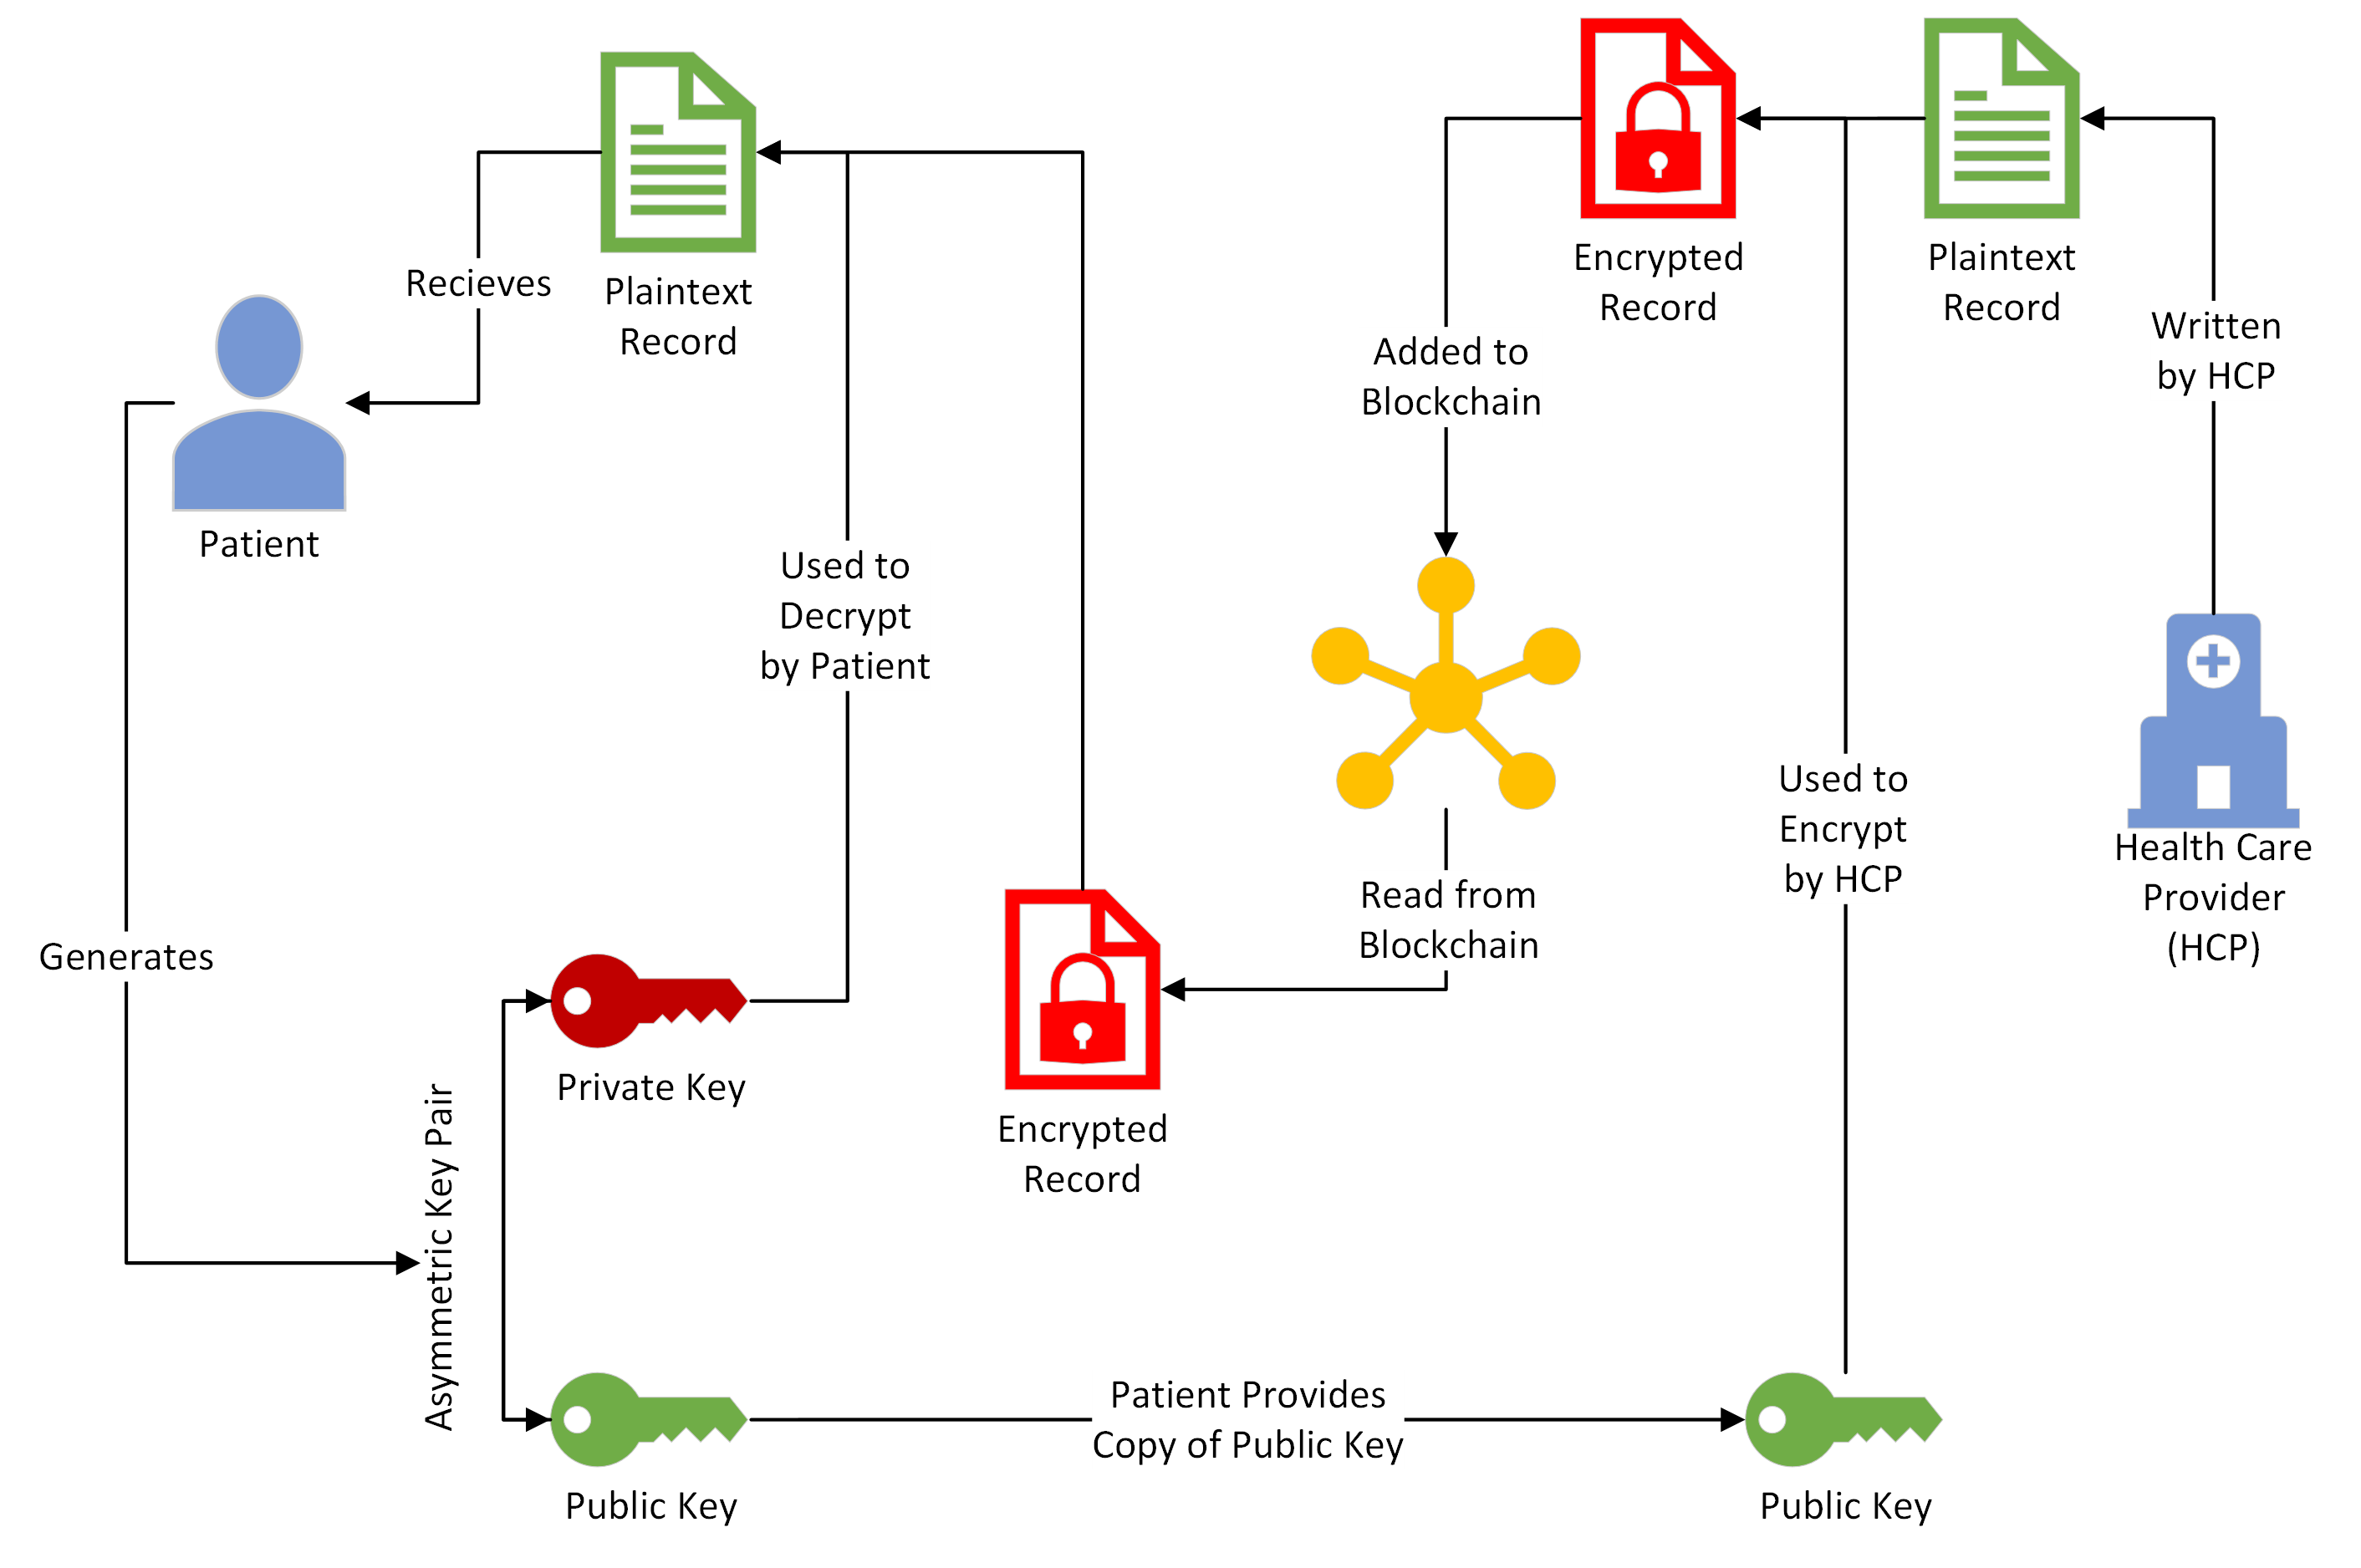
\includegraphics[width=\textwidth]{images/4990_encryption_structure.png}
\caption{A visual explanation of how public key cryptography is used to encrypt and decrypt records.}
\label{fig:encryption_decryption}
\end{figure}

\subsection{Networking}
\label{networking}
Our networking prototype involves two nodes: a doctor and a patient. In order for the doctor to view the patient's medical record, they must first request access from the patient. The doctor signs the transaction with their private key, which is then sent to the patient.

To decrypt the transaction, the patient must use the doctor's public key. The patient has an authorized list of doctors with their corresponding public keys, which allows them to decrypt the signatures of the doctor(s) they have authorized to view their records. If the patient cannot verify the signature, the transaction is closed and no data is sent to the doctor. However, if the patient can verify the signature, they can then decrypt the data the doctor requested using their private key.

Once the data has been decrypted, it can be encrypted with the doctor's public key and sent back to the doctor, ensuring that any data sent between nodes is protected against anyone who intercepts the communications. Once the doctor receives the data that is now encrypted using their public key, they can decrypt it using their private key.

Due to the limited nature of our networking implementation, there is further discussion of points where it can be expanded upon in Section \ref{improvements:networking}. 
% A smart contract implementation for a feature similar to what is described in the current section is also provided in Algorithm \ref{array-sum}.

\begin{figure}[h]
\centering
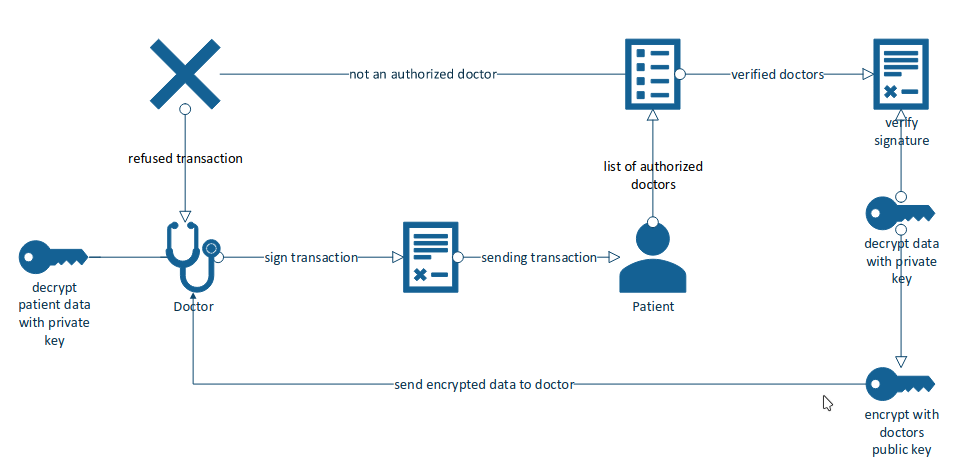
\includegraphics[width=\textwidth]{images/peer-to-peer.png}
\caption{Diagram showcasing our network's peer-to-peer connection}
\label{fig:peer-to-peer}
\end{figure}

\subsection{Frontend}
We created a basic application that can be accessed through a web browser. It splits functionality relevant to the two major user categories in a PHR system. For the purposes of our prototype there is no authentication, however in a production implementation it would be important to strictly control who is able to access each side.

\subsubsection{Provider Use Case}
Health care providers (HCPs) are able to use the app to add records (in the form of a block) to the blockchain, provided they are given the public key corresponding to a specific patient. A patient would need to send their public key to their HCP, which will be used to encrypt every field in the record before it is added to the blockchain. A transaction ID (in the form of a UUID) is then given to the doctor and will be used to identify the block where the encrypted cipher text will be stored. The HCP will need to give the transaction ID to the patient, preferably sending them back the public key file which has a section that stores a transaction log.

\subsubsection{Patient Use Case}
Patients are able to use the app to generate key pairs and view their health records. In order to view their data, they need a public key file, a private key file, and their public key file needs to have a list of transaction ids. The transactions are then decrypted and shown to the user in a table that allows them to filter and search data.

\subsection{Limitations and Considerations}

There are several aspects to consider regarding the limitations of our PHR system. Some of these limitations are due to choices we made, whereas others are unavoidable consequences of blockchain technology.

\subsubsection{Scalability}
Scalability refers to a blockchain's ability to handle increasing transaction volume and data storage as the blockchain grows. Scalability has been a significant challenge in the adoption of blockchain technology, as it can limit the number of transactions the network can process and increase the time required to validate new transactions.

Within our implementation, there are aspects that are not very scalable. As more blocks are added to the blockchain, the amount of time it takes to validate the blockchain will increase. The amount of time it takes to traverse the blockchain will also increase, which will affect users by increasing the amount of time it takes to locate all of their records.

Due to the chain being immutable, the disk-space required to host a node will only ever increase as more blocks are added. It could possibly get to the point where it is infeasible to host a copy of it on readily available hardware due to file size constraints.

As the number of users rises, the number of transactions per second will also rise. Alongside this, the amount of data needing to be stored and processed at any given moment will increase which could cause delays in transaction processing and validation, leading to slower network performance. Similarly, as the number of nodes rises there is the potential for network congestion which will possibly result in longer confirmation times and a decrease in network performance.

Further discussion of scalability and potential solutions can be found in \ref{industryanalysis:scalability}

\subsubsection{Mutability}
Our implementation features an intentionally immutable blockchain. We designed it this way in order to ensure the authenticity and integrity of the records. Is it not possible to forge or alter records once they have already been added to the blockchain, thus reducing chances for fraud and deception to occur.

However, this is not a foolproof implementation. There are valid reasons why mutability can be desirable within a PHR system.

\begin{itemize}
    \item Correcting mistakes in place is not possible. The only thing that can be done is create a new record with the fixes stored in it, however this will take up additional storage space on the blockchain.
    \item If a patient's private key is compromised, there is no way to protect their data from being accessed and read. If someone publicly releases a patient's private key, the entirety of their medical records will be publicly accessible for perpetuity.
    \item An immutable blockchain makes it so that the fields and data types are unchanging. We will be unable to introduce new fields that may eventually become necessary in the medical field.
\end{itemize}

\subsubsection{Encryption}
\label{limitations:encryption}
We have chosen to use RSA-4096 to encrypt patient records for reasons of convenience, but our implementation can be easily adapted to other encryption standards. However, there are some downsides to our current approach, which we outline below.
\begin{itemize}
    \item RSA encryption is vulnerable to attacks using quantum computers. If quantum computing technology advances to the point where it can readily crack RSA-4096, then our records may be compromised. This could be particularly problematic since blockchain records are immutable and cannot be changed retroactively. The details of how quantum computing might be able to do this are beyond the scope of this paper.
    \item RSA is relatively slow in some cases compared to the encryption and decryption speeds of other algorithms, such as elliptic curve cryptography (ECC).
    \item The size of our keys have to be large, which results in larger key file sizes and higher encryption and decryption times.
\end{itemize}

Additionally, the use of public key cryptography has downsides. Users must take care not to publicize their private keys. Users must also take active care to protect their private keys from theft or unauthorized access. If their private key is acquired by a malicious third party, all of their records will be made available to that third party. Since the blockchain is immutable, there is nothing that can be done to revoke their access to the patient's data.

\subsubsection{Usability and Security}
A blockchain based PHR system has many privacy, security, and patient autonomy benefits, however the level of knowledge and experience required to use our blockchain system is higher than what is ideal. In many jurisdictions, patients are not accustomed to having any sort of digital health records let alone blockchain based technology. It will be difficult to ease the transition into this sort of system for those who are older and less technologically savvy. We attempted to make our implementation as user-friendly as possible and added clear instructions, but there may be gaps in our implementation. In order to seriously assess the feasibility of a given implementation extensive quality assurance testing must be completed by a wide array of individuals to reduce the chances of patients being left out and unable to use the system.

This is also a security concern, as uncertain users might be more likely to take security risks such as exposing their private key information to unauthorized or malicious actors. According to the Anti-Phishing Work Group, the third quarter of 2022 set the highest record for the number of recorded phishing attacks \cite{www.apwg.org_2022}. They note that the number of phishing attacks has been rising. Our PHR system is reliant on public key cryptography where the user must keep their key private at all costs. If it is seen by a phisher, the entirety of a patient's medical records could be accessed and read. There would be no way to recover from this aside from generating a new key-pair for use in new records (all previous records would be permanently accessible to anyone with the original private key).

We are also limited by internet connectivity. Patients who are unable to gain access to the internet would be unable to view their medical records. As global internet connectivity is still less than 70\% (\cite{itu_2022}) of the global population, it is important to note that it will be impossible to implement such a system globally until global factors such as internet connectivity and political instability are addressed. 

Another factor to consider is the format of our frontend, we designed it with desktop computer sensibilities in mind. There is a large subset of users that are only on mobile platforms, which is not something our design was intended to be used on. In order to provide a more seamless experience, we would need to design our systems to support as many platforms as is possible.

\subsubsection{Node Host Incentives}
\label{node_incentives}
A major limitation of our PHR system is the lack of incentive for individuals or organizations to host additional nodes. Without a sufficiently distributed network, the blockchain becomes vulnerable to centralization and may compromise the integrity of the system.

Hosting a node may require potentially significant resources such as processing power and storage, resulting in high operating costs. The benefits of hosting a node are not always readily apparent to users, so they may not understand how vital it is for there to be many hosts for the security and reliability of the blockchain. Additionally, an absence of financial or other incentives can make it difficult to attract and retain node hosts.

Potential solutions to this issue would be to provide financial incentives to hosts. If a PHR was subsidized by governments, they could provide minor tax benefits to node hosts proportional to the amount of computational resources they provide. Alternatively, node hosts could receive compensation in the form of tokens or other cryptocurrencies. A downside of financial incentives is that it may result in attracting nodes who are primarily motivated by profit and are not interested in the interests of the system.

Another approach is to offer non-financial incentives to node hosts. For example, node hosts could be given a greater say in the governance of the PHR system, including voting rights and a voice in the decision-making process. However, this would have to be considered very carefully as to not silence the needs of those that cannot afford to contribute to the network.

Overall, creating incentives for individuals and organizations to host nodes is critical for the integrity and security of a production PHR. By implementing a compelling incentive scheme, we can attract a wide range of participants to create a distributed network that is resilient against centralization and other security threats.  

\subsubsection{Legal Considerations}
In addition to the security and privacy concerns discussed previously, it should also be noted that there is an ethical and legal dimension to the issue as well. Due to the immutable nature of the blockchain, it is impossible for data to be removed from it. This may have legal consequences in locations such as the European Union (EU) where they have the General Data Protection Regulation (GDPR) which requires services operating in the EU to give users the ability to have all of their data deleted \cite{GDPR-Art17}. This is not possible to implement in a decentralized blockchain, which may make it impossible to legally deploy this technology in the EU \cite{info:doi/10.2196/25094}.

\subsubsection{Networking Implementation}
\label{improvements:networking}
Our blockchain-based PHR system is decentralized which means that there is no central node/network that users will connect to. Instead, users become nodes themselves by hosting a copy of the blockchain and connecting to other nodes. Nodes would usually mine or listen in on other nodes. Mining is the process of adding a new block to the blockchain by performing computational work, in our case proof of work, to validate transactions and create new blocks. When a node makes a request to add a block, all the active nodes will do proof of work on that block (mining) and whomever finishes first would ideally be rewarded with some cryptocurrency or other incentives as discussed in Section \ref{node_incentives}. This mining process helps strengthen the integrity and security of the network by ensuring only valid transactions are added to the blockchain.


\begin{figure}[h]
\centering
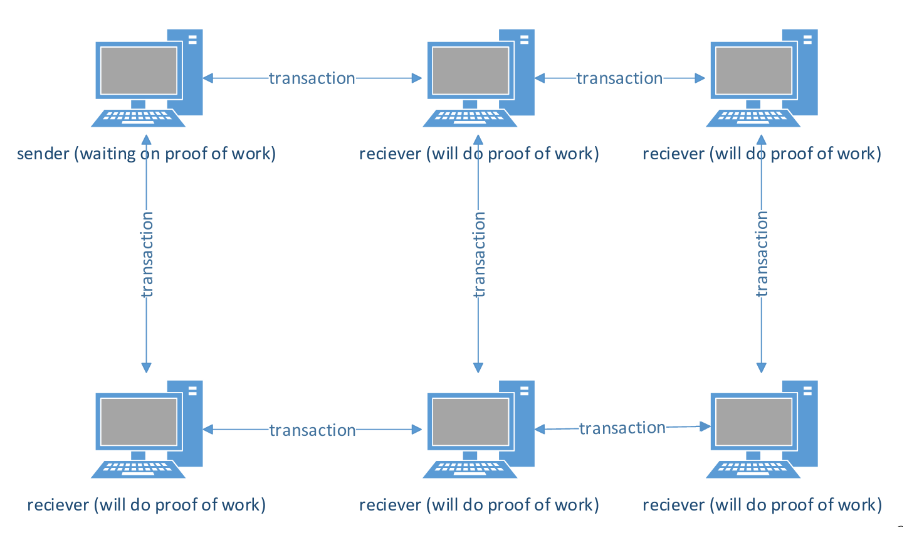
\includegraphics[width=\textwidth]{images/network.png}
\caption{This diagram provides a visual representation of how a decentralized PHR blockchain network would operate.}
\label{fig:network_diagram}
\end{figure}


\subsection{Intended Use Case}
From our analysis of the functionality and limitations of our system, we believe that it is best to be used alongside a traditional health record database. Blockchain-specific benefits like patient autonomy over their own records will be limited, however we do not currently have solutions in place to overcome the major limitations of our system as discussed in the previous section.

Having a blockchain-based "mirror" (new records would be inserted to the regular database as well as automatically encrypted then added to the blockchain) of medical health records that is opt-in would overcome many of the limitations discussed in the previous section. The opt-in nature of it might make it so that less technically savvy individuals are less likely to use the system, thus reducing the chances of user error. A smaller network would also mean less concerns relating to scalability and less compute resources would be required to keep the blockchain operational. An opt-in system might also help build trust in the blockchain-based PHR system for patients who might end up being interested in using it but would not be satisfied if they were forced into using it.

Having the blockchain system implemented in parallel will still bring many benefits, including giving patients the ability to be certain that their data is stored in a location which is immutable. While the database has the potential to be altered, a patient who is unsure of the validity of their medical records in the database can always check with the data on the blockchain to ensure that their records have been unaltered from the moment they were posted. 

There are still potential downsides of this approach, the greatest of which is cost. It will cost a lot more to run two redundant systems than it would to just run one. This approach should be considered for implementation in stable environments with the financial capacity to support two systems in parallel. Additionally, patients would also still have to make sure that their key is kept hidden from outsiders, otherwise their data will be permanently compromised as described previously.



% \subsubsection{Smart contract Implementation}
% Algorithm \ref{array-sum} presents an example implementation of a smart contract for a PHR blockchain system.
% % \begin{algorithm}
% % \caption{Doctor Signature Authorization Smart Contract Pseudocode}
% % \label{array-sum}
% % \begin{algorithmic}[1]
% % \Procedure{SmartContract}{$A$}
% %     \State $authorizedDoctors = $ list of authorized doctors
% %     \Function {CheckSignature}{signature}
% %         \If {doctor in authorizedDoctors}
% %         \EndIf
        
% %         \State Return $sum$
% %     \EndFunction
% % \EndProcedure
% % \end{algorithmic}
% % \end{algorithm}

% This implementation can be customized to fit different requirements/regulations, making it a versatile solution for PHR management.

\section{Industry Analysis}
Blockchain-based PHR systems are a rapidly evolving area of research, with new findings emerging constantly. These systems have been gaining popularity due to their potential to address several long-standing issues in healthcare data management. Research papers we have cited use a decentralized blockchain, although some opt for a centralized system that is more similar to our current infrastructure. In this section take a look at the limitations and benefits of using a blockchain PHR system. 
% TODO: analyze status of industry
\subsection{Scalability}
One of the main limitations of a blockchain PHR b system is scalability. Scalability is a crucial factor in the context of blockchain as it determines the ability of a blockchain network to process a large number of transactions and store vast amounts of data. Scalability has always been a topic of debate in the blockchain community, particularly when it comes to decentralized blockchains, which are immutable and store all data permanently.


It is a critical consideration when designing blockchain systems for medical records, as the size and complexity of the data being stored can significantly impact system performance. For example, the storage, encryption, and decryption of large medical images on the blockchain can consume significant computational resources, resulting in longer access times for users. Additionally, as the number of users on the blockchain grows, transaction verification times can increase exponentially, leading to potential performance issues. This is due to the blockchain's immutable nature, which requires each transaction to be verified and recorded on the ledger, making it increasingly difficult to process transactions as the system grows. Another challenge in achieving scalability is ensuring that data can be efficiently streamed to different devices, especially in a distributed network where nodes may have varying bandwidth and processing capabilities. Addressing these scalability concerns is critical for the successful implementation of blockchain-based PHR systems. Overall establishing a decentralized PHR blockchain can be a challenging task, especially for the long term where the system will continue to grow in size. This growth will make it increasingly difficult for transactions to be verified. This is an important aspect to consider for the future of blockchain technology.

\subsubsection{Off-chain storage and processing}
Off-chain storage is a potential solution some take to enhance there blockchains scalability. off-chain storage is storing data off of the blockchain. Usually in the form of an InterPlanetary File System (IPFS) or a secure database. It allows certain data or functions to be processed outside of the blockchain network. This frees up resources and allows for faster transaction processing. This can significantly increase the efficiency of the network and decrease transaction fees. An example would be storing medical images on an IPFS. Instead of storing this data off-chain, it can be encypted and stored off-chain inside an IPFS. If a health care provider where to request a patients records, the blockchain would only do the verification process (through a smart contract), the decryption and delivery of the data would be done off-chain. Essential this approach takes the task of storing and processing data, delegates it to an off-chain system, and the blockchain keeps track of who has authorization to view this data. 

The use of off-chain storage/processing also introduces potential issues that must considered. A major concern is the privacy and security risk that off-chain storage may introduce. Since Off-chain storage may not follow the same security protocols that a blockchain would, It also may not be immutable in nature and data may be deleted or edited. For those who want a completely decentralized and immutable approach this can be a deterrent. 

Data availability is another concern. Depending on the specific off-chain storage solution, a third-party might be introduced that would manage or maintain the infrastructure. For example, a hospital may have control over the off-chain data and could edit or remove data, which could compromise data privacy and security. While this approach can be beneficial in terms of scalability and efficiency, it can also compromise data privacy as other nodes would not be able to ensure that the data has not been tampered with. This is a common theme, in order to increase privacy and security, scalability needs to be sacrificed and vise-versa. Overall, while off-chain storage may be a solution for some, it comes with certain costs that users my not be willing to compromise on.

\subsection{Privacy}
While a blockchain can provide strong security, anonymity and immutability, this can also be a double-edged sword. A decentralized blockchain is immutable, which means that once a patient's record is on the chain, it cannot be removed. Patients are unable to erase their records, which  not only goes against the patient's wishes but it also goes against the regulations of the GDPR. The GDPR states that a patient should have the right to data erasure in article 17 (\url{https://gdpr-info.eu/art-17-gdpr/}). As a result there is an ongoing legal and ethical debate surrounding the use of blockchain-based PHR systems. Also, when it comes to storing data such as medical records, there is a significant demand for proper security measures to be taken to ensure the anonymity of the patients.

\subsubsection{Data breaches}
A potential privacy concern in a blockchain-based PHR system is related to data breaches. Since the blockchain will be immutable, the data stored on the chain will remain there permanently. For a PHR this information may include, names, age, addresses and medical history. This information can be used to easily identify a person. Attackers may find vulnerabilities in the system which can allow them to gain access to this sensitive information. This can be avoided by implementing strong encryption protocols and a strong decentralized network with a diversified set of nodes to prevent 51 percent attacks. Additionally patients must be educated on the importance of keeping there private key secure and how to identify/avoid phishing attacks.

\subsubsection{Patient information}
Another issue is incomplete patient information. In most blockchain-based PHR systems, patients are responsible for maintaining their own medical records, there is no authority that can verify the accuracy of there medical records. This could lead to misdiagnosis or incorrect treatment. One way to address this issue is by only giving health care providers the ability to diagnosis patients, as done in our implementation. By giving patients control over their medical records, they can choose to grant or deny access to healthcare providers. This empowers patients to maintain privacy with there information, while also entrusting that their medical records contain accurate information.


\subsection{Usability}
As a relatively new technology, a Blockchain system can be challenging for non-technical users to understand and fully utilize. This could lead to lose of access or theft of sensitive data. Furthermore verification time of each transaction can be slow due to the decentralized nature of the blockchain. Transaction times will continue to increase slowing down the process of accessing or updating patient records. Another significant issue is interoperability - blockchain-based PHR systems are still a new area of study and would need to establish a standard protocol or format for storing/exchanging data. Failure to address this could lead to difficulties in different systems  communicating with each other, limiting the usefulness of a blockchain-based PHR system in a broader healthcare context.

\subsubsection{User Interface}
User Interfaces (UIs) play a crucial role in the usability of any technology, especially PHR systems, as the user base can range from adults to the elderly. Blockchain technology, in particular, can be complex and difficult for non-technical users to understand. A poorly designed UI can exacerbate the difficulties that users face with an already complex system. A well-designed UI can guide users on how to generate keys and manage there health records, as demonstrated in our implementation. Including a manual/instructions page can further facilitate users' navigation and understanding of this new technology, helping to promote a health ecosystem and keeping patients connected to the decentralized network. A lack of a proper UI may discourage users from using a blockchain-based PHR system, instead preferring to rely on traditional healthcare providers to manage their records, as is currently the case.

\subsubsection{Key management}
Key management is an essential aspect of any blockchain system, especially for blockchain-based PHR systems. Blockchains rely on cryptographic keys to secure the data. Users must securely manage their private key in order to maintain control over there medical records, this can be difficult for users to manage. One of the challenges of key management is to maintain a balance between usability and security. A patient needs to ensure hat their private key is stored securely o prevent unauthorized access to their data. This process of securely storing and managing a private key may be complex and burdensome for some patients. If users are not educated about key management it can lead to a loss of access to their medical records. Overall we need to ensure that users are educated on best practices for managing their private keys.


\subsection{A new use case}
The research we have studied look at the PHR blockchain system as a possible replacement to our current infrastructure.

\label{industryanalysis:scalability}
% explain how scalability has been addressed by other implementations
% talk about sharding and off chain databases
% TODO: tradeoff triangle

\section{Conclusion}
% TODO: write conclusion
\printbibliography
\end{document}
